% https://www.staples.com/services/printing/posters/
% $20 off poster orders of $70 or more. Coupon code 84987. Expires 1/3/26.

\documentclass[portrait,a0b,final,a4resizeable]{a0poster}

\setlength{\paperwidth}{36in}
\setlength{\paperheight}{48in}

\usepackage{atbegshi}% http://ctan.org/pkg/atbegshi
\AtBeginDocument{\AtBeginShipoutNext{\AtBeginShipoutDiscard}}

\usepackage[margin=0.5in]{geometry}
\usepackage{multicol}
\usepackage{enumitem}
\usepackage{mathtools}
\usepackage{amsmath, amsthm, amssymb, bm}
\usepackage{multirow}
\usepackage{nicematrix}
\usepackage{bussproofs}
\usepackage{wrapfig}
\makeatletter
\def\defaultHypSeparation{\hskip 65pt}
\def\extraVskip{6pt}
\makeatother
\usepackage{pgfplots}
\pgfplotsset{compat=1.18}
\usepackage{dsfont}
\usepackage{qrcode}
\usepackage{svg}
\usetikzlibrary{automata, positioning, arrows.meta}

%\setlength{\proofhsep}{55pt}   % default is smaller
%\setlength{\proofvsep}{50pt}   % optional

\usetikzlibrary{cd,shapes.geometric,arrows,chains,matrix,positioning,scopes,calc,trees}

\input{include/jlposter}
\usepackage{include/preamble}

% ----------------------------
% Paper/Poster notation
% ----------------------------
\definecolor{Light}{gray}{.90}
\usepackage{soul}
\sethlcolor{Light}

\makeatletter
\providecommand{\leftsquigarrow}{%
  \mathrel{\mathpalette\reflect@squig\relax}%
}
\newcommand{\reflect@squig}[2]{%
  \reflectbox{$\m@th#1\rightsquigarrow$}%
}
\makeatother

\newcommand{\codett}[1]{\texttt{\hl{#1}}}
\newcommand{\nt}[1]{\texttt{#1}}
\newcommand{\tok}[1]{\codett{#1}}
\newcommand{\gap}{\;\;}

\newcommand{\T}{\mathbb{T}}

\DeclareMathOperator*{\largecomma}{\mathop{\vcenter{\hbox{\Huge\texttt{,}}}}}
\newcommand{\cjoin}[2]{\mathop{\largecomma}\limits_{#1}^{#2}}
\newcommand{\jointspacing}{\vspace{0.3in}}

\newcommand{\bs}{\blacksquare}
\newcommand{\ws}{\square}

\begin{document}
\begin{poster}
  \vspace{1cm}

%%% Header (same structure)
  \begin{center}
    \begin{pcolumn}{1.03}
      \begin{minipage}[c][9cm][c]{0.85\textwidth}
        \begin{center}
        {\Huge \textbf{Weighted Automata Learning with a Hard Inductive Bias}}\\[8mm]
        {\huge Breandan Considine}
        \end{center}
      \end{minipage}
    \end{pcolumn}
  \end{center}

  \vspace*{-0.5cm}
  \large
  \Large

  \begin{multicols}{2}

% =========================================================
    \mysection{Main Idea}

    \vspace*{-0.8cm}
    \null\hspace*{2.8cm}\begin{minipage}[c]{0.86\columnwidth}
          \renewcommand\labelitemi{$\vcenter{\hbox{\small\bullet}}$}
          \begin{itemize}
            \labelsep=0.8cm
%            \itemindent=-0.6cm
            \item \textbf{Assume}: we are given a learned distribution, $P_{\theta}(\sigma)$, with support over $\sigma: \Sigma^+$ but largely concentrated within $\mathcal{L}(G)$, where $G$ is a known CFG.
            \item \textbf{Our goal}: distill a surrogate WFA, $\alpha_{\hat\theta}$, such that for all $\sigma \in \mathcal{L}(G)$, $P_{\hat\theta}(\sigma) \propto P_{\theta}\big(\sigma \mid \sigma \in \mathcal{L}(G)\big)$, while preserving inclusion $\big(\mathcal{L}(\alpha)\supseteq \mathcal{L}(G)\big)$.
            \item \textbf{Desiderata}: Regular description $\alpha$ should be reasonably concise and precise, i.e., $\Delta = |\mathcal{L}(\alpha) \setminus \mathcal{L}(G)|$ is approximately minimized up to $\Sigma^n$.
          \end{itemize}
    \end{minipage}

    \jointspacing

% =========================================================
\mysection{Nederhof's Regular Approximation}

\null\hspace*{2.8cm}\begin{minipage}[c]{0.87\columnwidth}
  A recursive transition network (RTN) of a CFG $\langle \Sigma,V, P, S\rangle$ is an automaton,
  \[
    \mathcal R=\big\{R_A=(Q_A,\delta_A,\alpha_A,F_A)\big\}_{A\in V},
    \:\:
    \delta_A\subseteq Q_A\times\big(\Sigma\cup V\cup\{\varepsilon\}\big)\times Q_A,
  \]
  where an arc labelled \(B\in V\) denotes a call to \(R_B\). For example, consider the CFG, $\texttt{S } \rightarrow \texttt{ x } \mid \texttt{ S S } \mid \texttt{ \{ S \}}$, which has the following RTN:

  % https://dreampuf.github.io/GraphvizOnline/?engine=dot#digraph%20RTN_S%20%7B%0A%20%20%20%20rankdir%3DLR%3B%0A%20%20%20%20nodesep%3D0.3%3B%0A%20%20%20%20node%20%5Bshape%3Dcircle%2C%20fontname%3D%22JetBrains%20Mono%22%2C%20fontsize%3D12%5D%3B%0A%20%20%20%20edge%20%5Bfontname%3D%22JetBrains%20Mono%22%2C%20fontsize%3D10%5D%3B%0A%0A%20%20%20%20entry%20%5Blabel%3D%22%22%2C%20shape%3Dnone%2C%20width%3D0%5D%3B%0A%20%20%20%20s_S%20%20%20%5Blabel%3D%22q0%22%5D%3B%0A%20%20%20%20f_S%20%20%20%5Blabel%3D%22qf%22%2C%20shape%3Ddoublecircle%5D%3B%0A%0A%20%20%20%20entry%20-%3E%20s_S%3B%0A%0A%20%20%20%20s_S%20-%3E%20f_S%20%5Blabel%3D%22%20x%20%22%5D%3B%0A%0A%20%20%20%20s_S%20-%3E%20q1%20%5Blabel%3D%22%20S%20%22%2C%20color%3Dblue%2C%20penwidth%3D2.0%5D%3B%0A%20%20%20%20q1%20%20-%3E%20f_S%20%5Blabel%3D%22%20S%20%22%2C%20color%3Dblue%2C%20penwidth%3D2.0%5D%3B%0A%0A%20%20%20%20s_S%20-%3E%20q2%20%5Blabel%3D%22%20%7B%20%22%5D%3B%0A%20%20%20%20q2%20%20-%3E%20q3%20%5Blabel%3D%22%20S%20%22%2C%20color%3Dblue%2C%20penwidth%3D2.0%5D%3B%0A%20%20%20%20q3%20%20-%3E%20f_S%20%5Blabel%3D%22%20%7D%20%22%5D%3B%0A%7D

  \begin{center}
%  \includegraphics[width=0.65\linewidth]{rtn.png}
    \hspace{-3cm}
    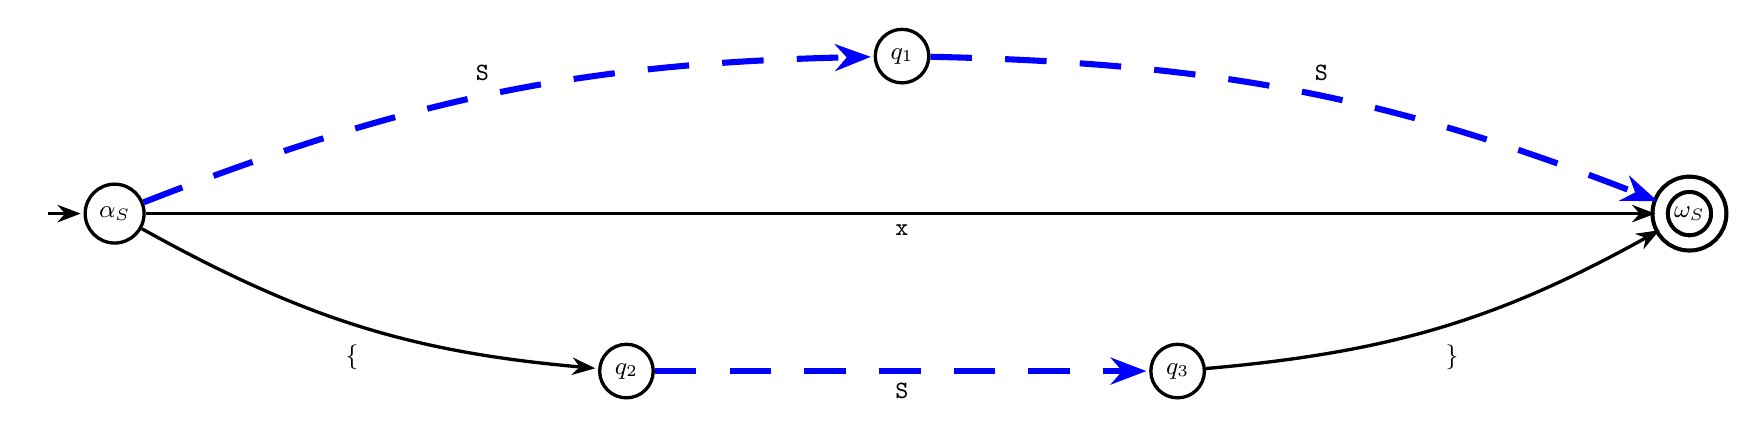
\begin{tikzpicture}[
  shorten >=1pt,
  on grid,
  >=Stealth,
  initial text=,
% 1. Bolder nodes with smaller diameter
  every state/.style={
    draw,
    circle,
    font=\small\ttfamily,
    minimum size=0.6cm,
    line width=1.2pt
  },
% 2. Thick standard edges
  every edge/.append style={
    line width=1.2pt
  },
% 3. Extra thick blue dashed edges (corresponds to original penwidth 2.0)
  rtn_call/.style={
    draw=blue,
    dashed,
    line width=2.2pt
  },
  label_font/.style={
    font=\small\ttfamily
  },
% 4. Final state with clear 2pt separation gap
  accepting/.style={
    state,
    double,
    double distance=4pt,
    line width=1.5pt % Thickness of the two individual circles
  }
]

  % Grid-aligned Nodes (Total Width: 12 units)
  \node[state, initial] (q0) at (-3, 0) {$\alpha_S$};
  \node[state, accepting] (qf) at (17, 0) {$\omega_S$};

  % Top path (Recursive S calls)
  \node[state] (q1) at (7, 2) {$q_1$};

  % Bottom path (Brackets)
  % Increased horizontal distance from q0 to q2 and q3 to qf
  \node[state] (q2) at (3.5, -2) {$q_2$};
  \node[state] (q3) at (10.5, -2) {$q_3$};

  % Edges
  \path[->]
  % Base case transition
  (q0) edge node[below, label_font] {x} (qf)

  % Top recursive path: S -> S
  (q0) edge[rtn_call, dash pattern=on 15pt off 12pt, bend left=10] node[above left, label_font, black] {S} (q1)
  (q1) edge[rtn_call, dash pattern=on 15pt off 12pt, bend left=10] node[above right, label_font, black] {S} (qf)

  % Bottom bracket path: { -> S -> }
  % Higher bend and wider horizontal spacing for better label clearance
  (q0) edge[bend right=12] node[below left=0.1cm and -0.1cm, label_font] {\{} (q2)
  (q2) edge[rtn_call, dash pattern=on 15pt off 12pt] node[below, label_font, black] {S} (q3)
  (q3) edge[bend right=12] node[below right=0.1cm and -0.1cm, label_font] {\}} (qf);

\end{tikzpicture}

  \end{center}

  % https://arxiv.org/pdf/cs/9910022#page=8

  \textbf{Nederhof's \(d\)-RTN approximation} is a depth-bounded RTN unfolding. A nonterminal arc \(p \overset{B}{\longrightarrow} q\) is replaced by a fresh copy of the RTN for \(B\), adding \(\varepsilon\)-arcs from \(p\) to the copy's initial state and the copy's final state back to \(q\): \( p \overset{\varepsilon}{\longrightarrow} \alpha_B', \:\: \omega_B' \overset{\varepsilon}{\longrightarrow} q \quad(\forall \omega_B'\in F_B')\). Unfold calls for \(d\) rounds. At depth \(d\), every remaining nonterminal arc \(p\overset{B}{\longrightarrow}q\) is woven into a shared copy of \(R_B\): \( p \overset{\varepsilon}{\longrightarrow} \alpha_B, \:\: \omega_B \overset{\varepsilon}{\longrightarrow} q \quad(\forall \omega_B\in F_B) \). Below is the $\varepsilon$-removed, determinized and minimized DFA depicted for $1 \leq d \leq 4$:\vspace{0.5cm}

  \begin{center}
    \setlength{\tabcolsep}{0.15cm}
    \renewcommand{\arraystretch}{1.15}

    \begin{tabular}{@{}ccccccc@{}}
      \begin{minipage}{0.09\linewidth}
        \centering
        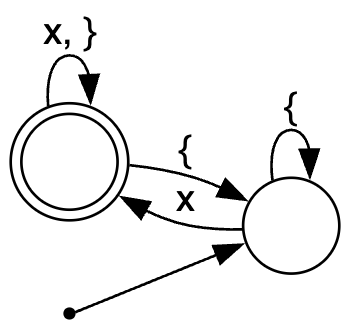
\includegraphics[width=0.85\linewidth]{d1.png}
      \end{minipage}
      &&
      \begin{minipage}{0.20\linewidth}
        \centering
        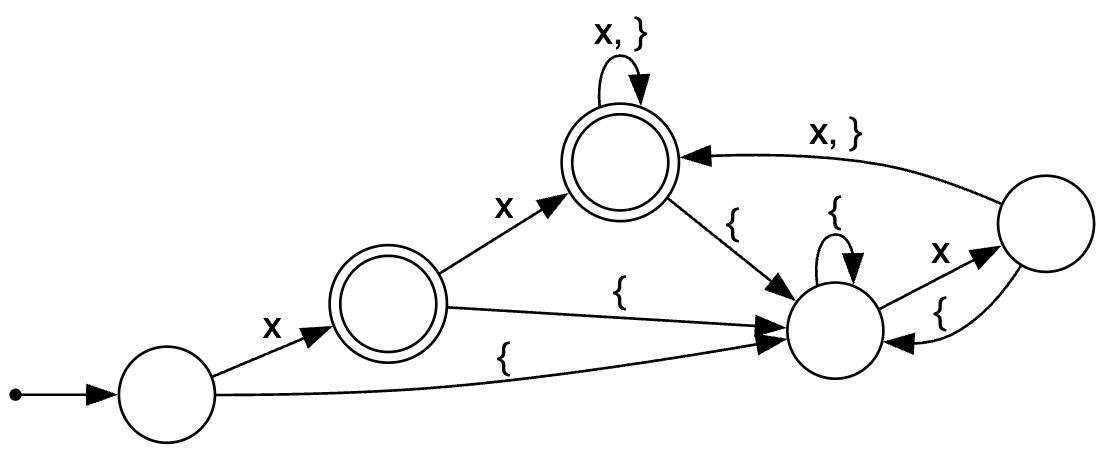
\includegraphics[width=\linewidth]{d2.png}
      \end{minipage}
      &&
      \begin{minipage}{0.26\linewidth}
        \centering
        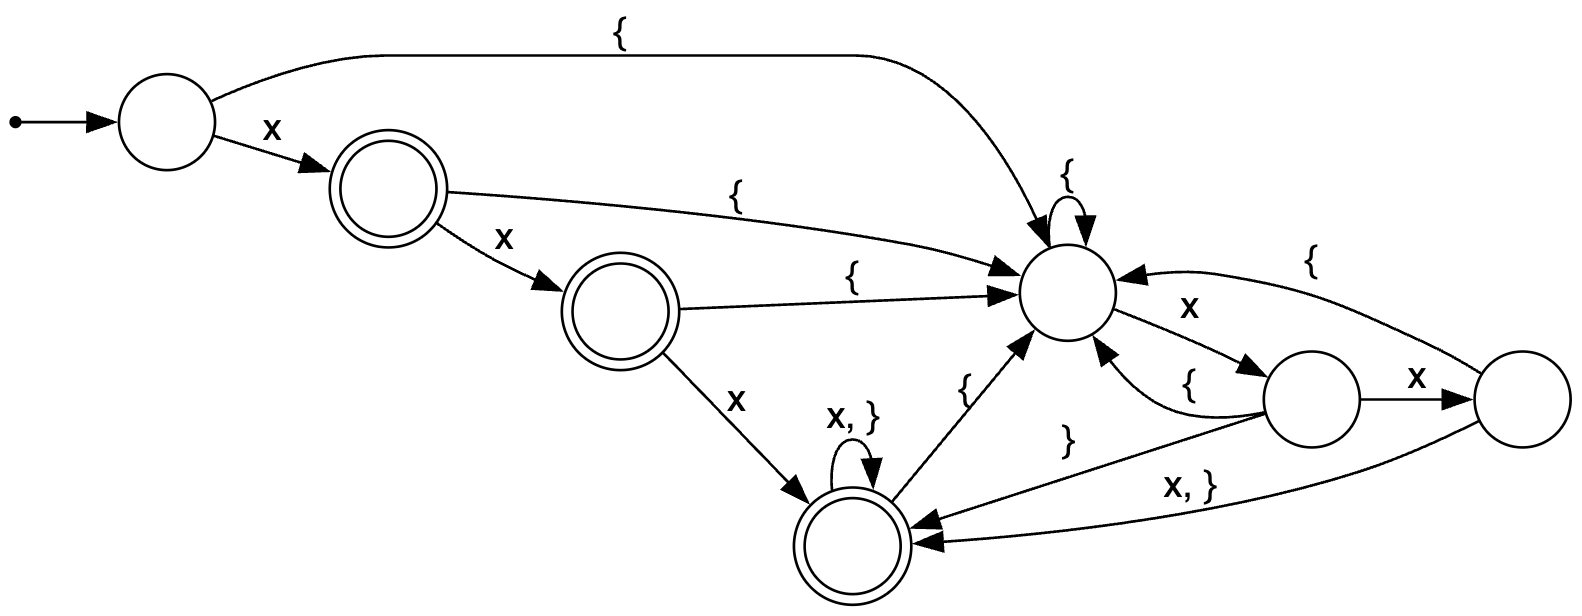
\includegraphics[width=\linewidth]{d3.png}
      \end{minipage}
      &&
      \begin{minipage}{0.38\linewidth}
        \centering
        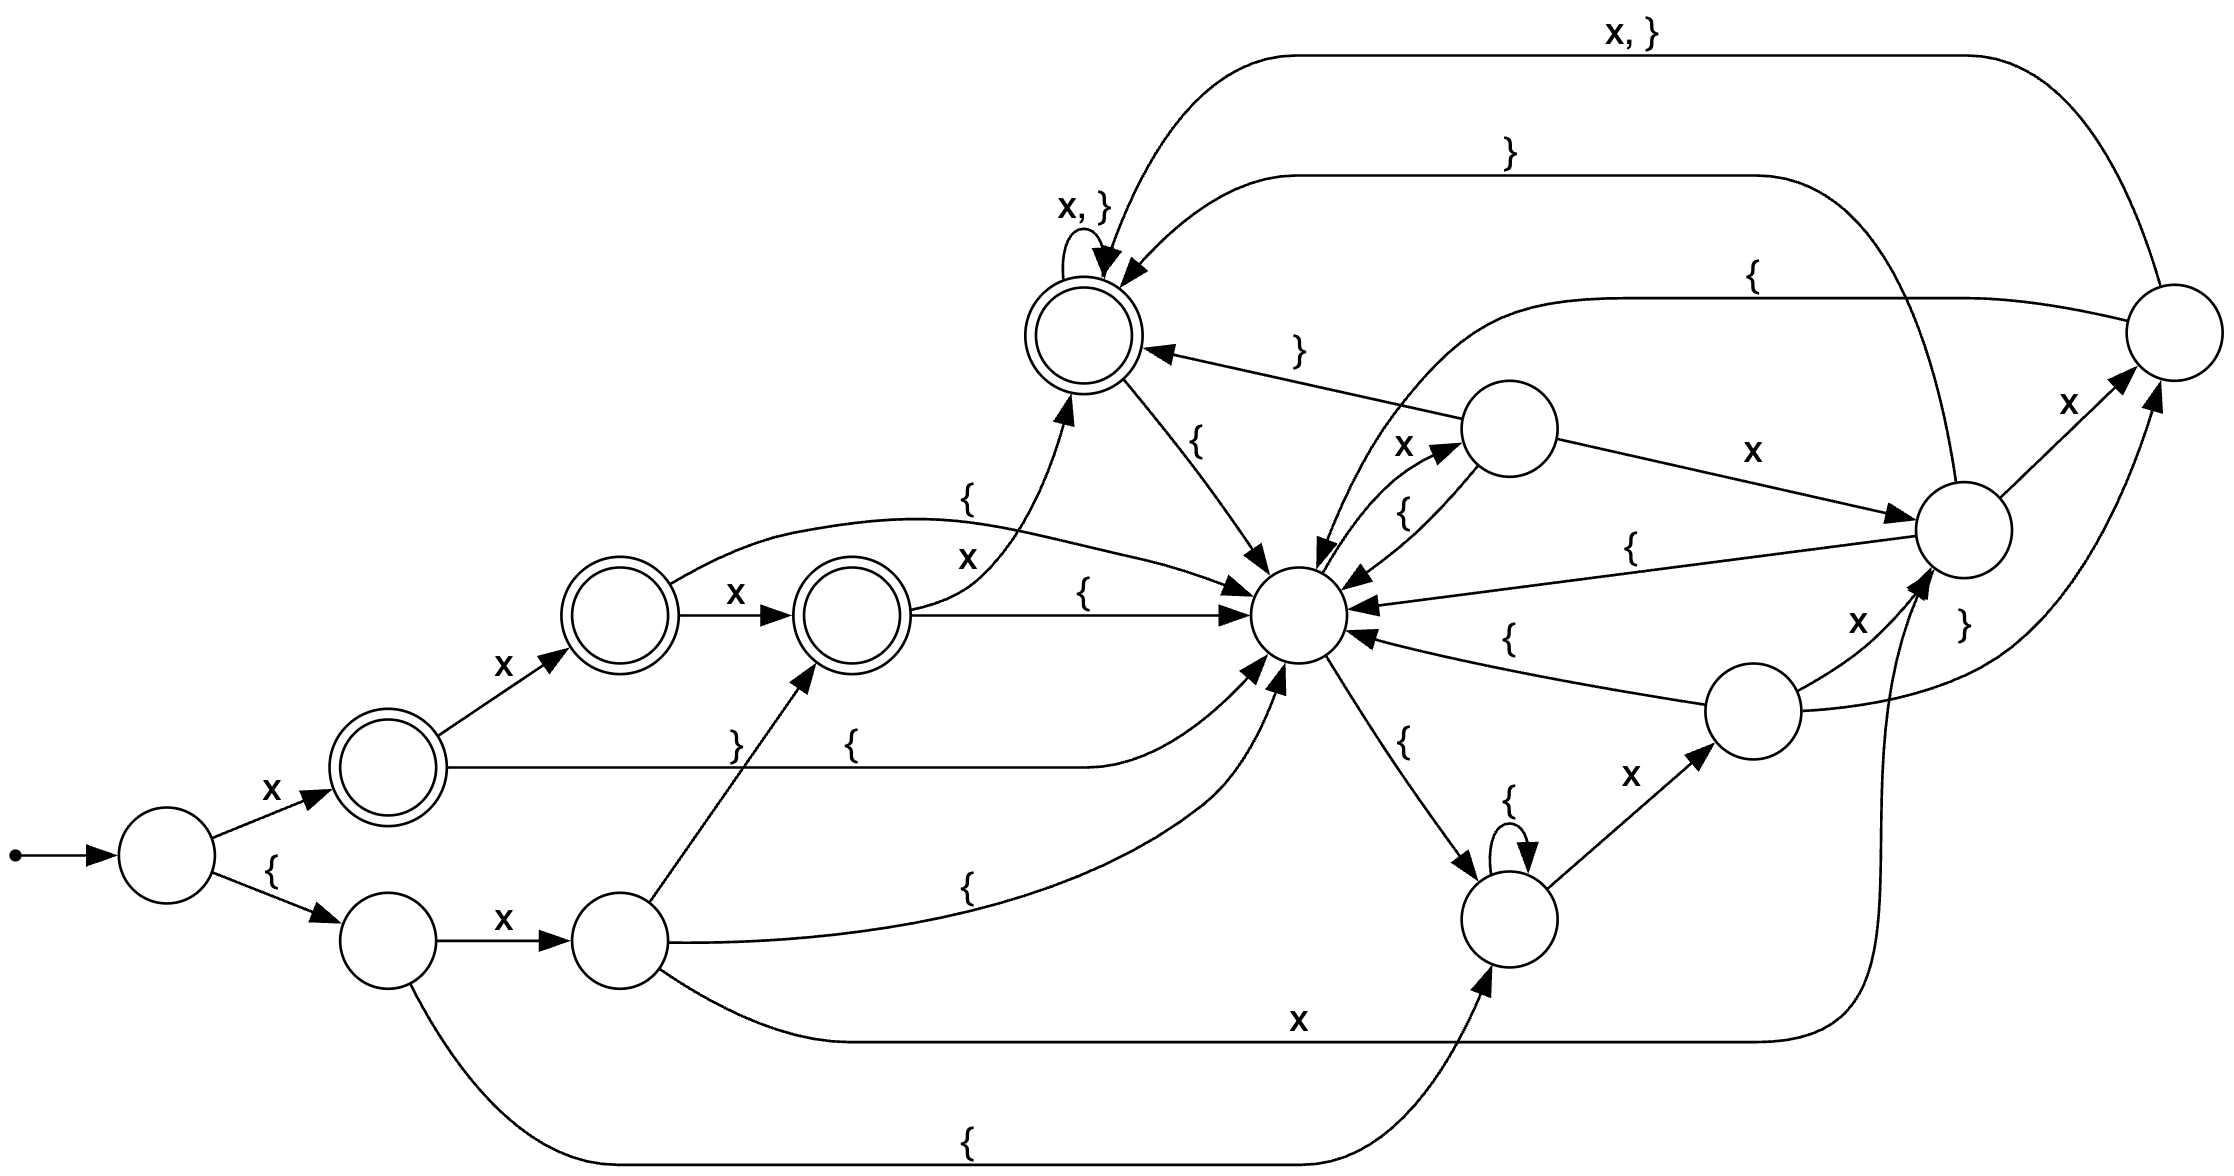
\includegraphics[width=\linewidth]{d4.png}
        \vspace{-0.9cm}
      \end{minipage}\\
      \textbf{$d=1$} && \textbf{$d=2$} && \textbf{$d=3$} && \textbf{$d=4$}
    \end{tabular}
    \vspace{0.1em}
  \end{center}
  \end{minipage}

    \jointspacing

    \mysection{Language Overapproximation}

    \vspace{0.7em}\hspace{0.5cm}
  \begin{minipage}[t]{0.35\linewidth}
    \centering
    \resizebox{0.9\linewidth}{!}{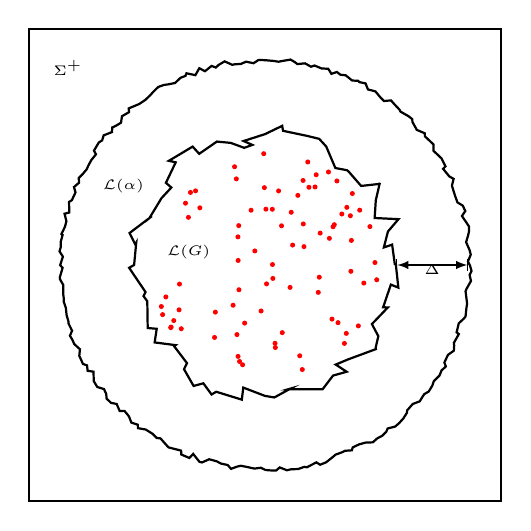
\begin{tikzpicture}[>=latex, every node/.style={font=\tiny}
]
  \coordinate (C) at (3,3);

  \draw[thick] (0,0) rectangle (6,6);
  \node at (0.5,5.5) {$\Sigma^+$};

  \pgfmathsetseed{12310}
  \begin{scope}[decoration={random steps,segment length=2pt,amplitude=1.02pt}]
    \draw[thick,decorate] (C) circle [radius=2.6];
  \end{scope}
  \node at (1.2,4.0) {$\mathcal{L}(\alpha)$};

  \begin{scope}[decoration={random steps,segment length=4pt,amplitude=4pt}]
    \draw[thick,decorate] (C) circle [radius=1.65];
  \end{scope}
  \node at (2.03,3.17) {$\mathcal{L}(G)$};

  \pgfmathsetseed{2673}
  \begin{scope}
    \clip (C) circle[radius=1.5];
    \foreach \k in {1,...,80}{
      \pgfmathsetmacro{\rr}{sqrt(rnd)*1.45}
      \pgfmathsetmacro{\tt}{rnd*360}
      \fill[red] ($(C)+(\tt:\rr)$) circle[radius=0.032];
    }
  \end{scope}
  % Calculate exact positions for the gap measurement line at 3 o'clock (0 degrees).
% We add a small 0.1em pad for the label and a small gap for clarity.
% For the outer circle, we use the un-decorated (minimum) radius.
  \coordinate (gap_start) at ($(C)+(0:1.65)$);
  \coordinate (gap_end) at ($(C)+(0:2.6)$);

% Draw the line with vertical bars and internal arrows
  \draw[|<->|, thin, shorten >=0.05em, shorten <=0.05em] (gap_start) -- (gap_end);

% Place the label \Delta above the line
  \node[anchor=south, yshift=-0.25cm] at ($(gap_start)!0.5!(gap_end)$) {$\Delta$};
\end{tikzpicture}}
  \end{minipage}
  \hspace{0.1cm}
  \begin{minipage}[t]{0.52\linewidth}
    \centering
    \resizebox{1.2\linewidth}{!}{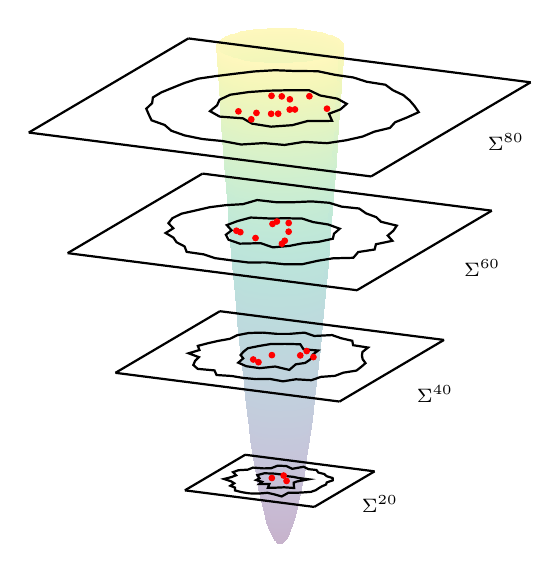
\begin{tikzpicture}
  \begin{axis}[
    view={25}{14},
    width=9.2cm,
    height=10cm,
    xmin=-10, xmax=10,
    ymin=-10, ymax=10,
    zmin=0, zmax=8,
    hide axis,
    grid=none,
  ]

    \pgfmathsetmacro{\R}{sqrt(8)}
    \addplot3[
    surf,
    shader=interp,
    opacity=0.3,
    colormap/viridis,
    domain=0:360,
    y domain=0:\R,
    samples=55,
    samples y=25
    ] ({y*cos(x)}, {y*sin(x)}, {y^2});

    \pgfmathsetseed{12310}

    \foreach \z [count=\zi] in {1,3,5,7}{

      \pgfmathsetmacro{\rinner}{sqrt(\z/0.9)}
      \def\innerpoints{}

      \foreach \sample in {1,...,20}{
        \pgfmathsetmacro{\ang}{360*\sample/20}
        \pgfmathsetmacro{\noise}{0.4 * rand}
        \pgfmathsetmacro{\xx}{(\rinner + \noise) * cos(\ang)}
        \pgfmathsetmacro{\yy}{(\rinner + \noise) * sin(\ang)}
        \xdef\innerpoints{\innerpoints (\xx,\yy,\z)}
      }

      \addplot3[black, thick] coordinates {\innerpoints} -- cycle;

      \pgfmathtruncatemacro{\seed}{2000+\zi}
      \pgfmathsetseed{\seed}

      \def\dotpoints{}
      \pgfmathtruncatemacro{\numdots}{3*\zi}

      \foreach \k in {1,...,\numdots}{
        \pgfmathsetmacro{\rr}{sqrt(rnd)*\rinner*0.9}
        \pgfmathsetmacro{\tt}{rnd*360}
        \pgfmathsetmacro{\xx}{\rr * cos(\tt)}
        \pgfmathsetmacro{\yy}{\rr * sin(\tt)}
        \xdef\dotpoints{\dotpoints (\xx,\yy,\z)}
      }

      \addplot3[red, only marks, mark=*, mark size=1] coordinates {\dotpoints};

      \pgfmathsetmacro{\rmid}{sqrt(\z/0.2)}
      \def\middlepoints{}

      \foreach \sample in {1,...,40}{
        \pgfmathsetmacro{\ang}{360*\sample/40}
        \pgfmathsetmacro{\noise}{0.3 * rand}
        \pgfmathsetmacro{\xx}{(\rmid + \noise) * cos(\ang)}
        \pgfmathsetmacro{\yy}{(\rmid + \noise) * sin(\ang)}
        \xdef\middlepoints{\middlepoints (\xx,\yy,\z)}
      }

      \addplot3[black, thick] coordinates {\middlepoints} -- cycle;

      \pgfmathsetmacro{\h}{sqrt(\z / 0.1)}

      \addplot3[black, thick] coordinates { (-\h,-\h,\z) (-\h, \h,\z) };
      \addplot3[black, thick] coordinates { ( \h,-\h,\z) ( \h, \h,\z) };
      \addplot3[black, thick] coordinates { (-\h,-\h,\z) ( \h,-\h,\z) };
      \addplot3[black, thick] coordinates { (-\h, \h,\z) ( \h, \h,\z) };
    }

  \end{axis}

  \path (current bounding box.north east) coordinate (plotNE);

  \node[font=\scriptsize, anchor=north west, inner sep=1pt]
  at ($(plotNE)+(-0.6,-1.3)$) {$\Sigma^{80}$};
  \node[font=\scriptsize, anchor=north west, inner sep=1pt]
  at ($(plotNE)+(-0.9,-2.9)$) {$\Sigma^{60}$};
  \node[font=\scriptsize, anchor=north west, inner sep=1pt]
  at ($(plotNE)+(-1.5,-4.5)$) {$\Sigma^{40}$};
  \node[font=\scriptsize, anchor=north west, inner sep=1pt]
  at ($(plotNE)+(-2.2,-5.9)$) {$\Sigma^{20}$};

\end{tikzpicture}
\hspace{-0.8cm}
\resizebox{0.25\linewidth}{!}{
  \begin{tikzpicture}
    % Image
    \node[inner sep=0pt, anchor=south west] (img) at (0,0)
      {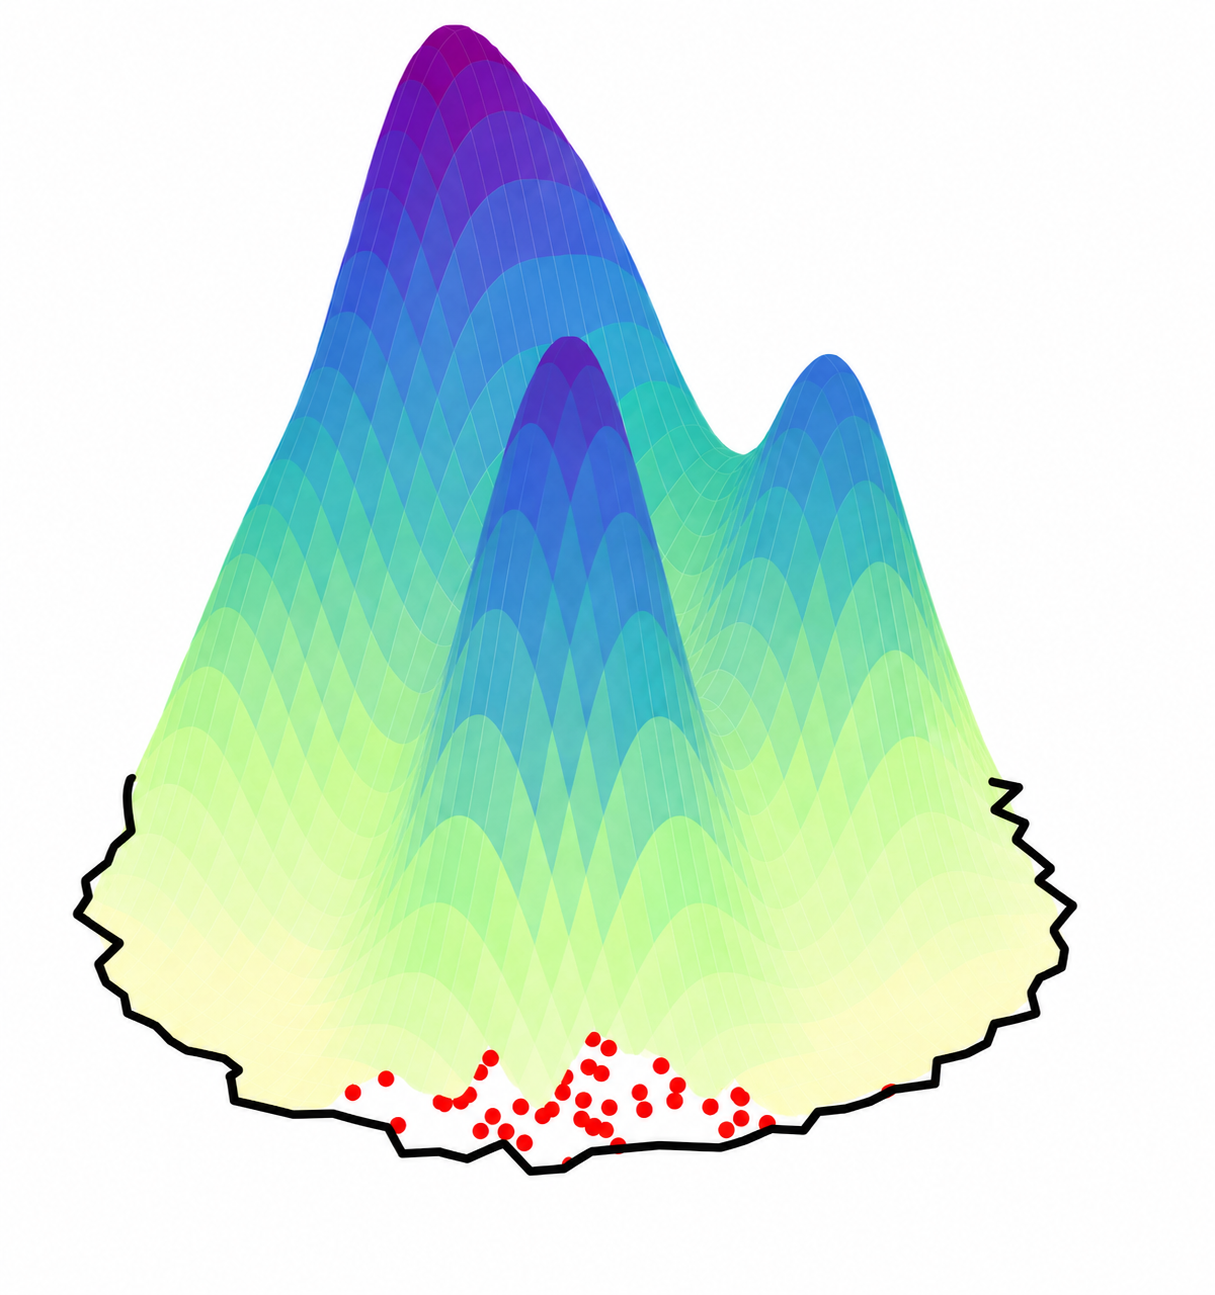
\includegraphics[width=0.3\linewidth]{plot.png}};

    % Title above image
    \hspace{-0.2cm}\node[anchor=south, font=\small\bfseries] at (img.north) {$P_\theta\big(\sigma \mid \sigma \in \mathcal{L}(G)\big)$};

    % Bottom-left label
    \node[
      anchor=south west,
      font=\small,
      fill=white,
      fill opacity=0.75,
      text opacity=1,
      inner sep=2pt
    ] at ([xshift=-0.4cm,yshift=0.03cm]img.south west)
      {$\mathcal{L}(G)$};
  \end{tikzpicture}
}}  \end{minipage}
  \vspace{0.3em}

    \null\hspace*{2.8cm}\begin{minipage}[c]{0.86\columnwidth}
  We can measure over-approximation tightness by considering finite models,\\
    \[
      \rho(\alpha, G, m) =
      \frac{\sum_{n=1}^m |\mathcal{L}(G)\cap\Sigma^n|}
      {\sum_{n=1}^m |\mathcal{L}(\alpha)\cap\Sigma^n|},
      \:\:\alpha \sqsubset_G^m \alpha'
      \iff
      \rho(\alpha',G,m) < \rho(\alpha,G,m).
    \]
  \end{minipage}
    \vspace{0.7em}

    \mysection{Our Method}

    \null\hspace*{2.8cm}\begin{minipage}[c]{0.86\columnwidth}
    We propose a counterexample-guided abstraction refinement (CEGAR) loop that incrementally refines $\alpha_{\hat\theta}$ until a desired precision or $|Q|_\max$ is reached:\vspace{0.4cm}
    \end{minipage}

    \begin{enumerate}
      \itemsep0em
      \itemindent=4cm
      \sloppy
      \setlength{\emergencystretch}{5cm}
      \item \phantom{.}Initialize $\alpha_{\hat\theta}'\leftarrow \alpha_d$ using Nederhof's $d$-RTN construction.
      \item \phantom{.}Propose a refinement $D_\text{KL}(P_{\theta}\|\alpha_{\hat\theta}) < D_\text{KL}(P_{\theta}\|\alpha_{\hat\theta}')$ and $\alpha_{\hat\theta} \sqsubset_G^m \alpha_{\hat\theta}'$.
      \item \phantom{.}Binarize $\alpha_\hat\theta$ and verify $\mathcal{L}(\alpha) \supset \mathcal{L}(G)$ by checking $\varnothing =\mathcal{L}(G)\cap \overline{\mathcal{L}(\alpha)}$.
      \item \phantom{.}If verification fails, collect $x \in \mathcal{L}(G)\cap \overline{\mathcal{L}(\alpha)}$, otherwise go to step 2.
      \item \phantom{.}Repair $\alpha$ restoring inclusion, renormalize as $\alpha_{\hat\theta}'$, then go to step 2.
    \end{enumerate}

    \jointspacing\newpage

% =========================================================
    \mysection{Maximum Probability Intersection Decoding}

    \vspace{-2.5cm}
    \null\hspace*{2.8cm}\begin{minipage}[t]{0.86\columnwidth}
      \begin{minipage}[t]{0.48\linewidth}\vspace{0pt}
        We will evaluate our learned WFA on a constrained decoding task: given a dataset of near-words $\err\sigma \notin \mathcal{L}(G)$ and pairwise repairs $\sigma$ within a small edit distance, sample uniformly WoR repairs within $\ell_\cap$, score and rank each repair according to $P_{\hat\theta}(\sigma)$, then measure mean reciprocal rank{\parfillskip=0pt\par}
      \end{minipage}%
      \hfill
      \begin{minipage}[t]{0.48\linewidth}
        \vspace{-0.2cm}
        \begin{center}
          \resizebox{\linewidth}{!}{\begin{tikzpicture}[
  scale=4.5,
  >={Stealth[length=12pt, width=10pt]},
  dot/.style = {circle, inner sep=0pt, minimum size=4mm, fill, node contents={}},
  posterline/.style = {line width=3pt}
]
  % 1. Draw the underlying layers
  \draw[posterline] (-2.1,0) coordinate (a) circle (2.4) node[dot,label={[font=\large]above left:$\err{\sigma}$}](z0);

  \draw [posterline, dash pattern=on 15pt off 12pt] (a) circle (0.6);
  \draw [posterline, dash pattern=on 15pt off 12pt] (a) circle (1.2);
  \draw [posterline, dash pattern=on 15pt off 12pt] (a) circle (1.8);

  \draw[->, posterline] (-2.1,0) -- (-1.5, 0) node[midway,below]{$d_1$};
  \draw[->, posterline] (-1.5,0) -- (-0.9, 0) node[midway,below]{$d_2$};
  \draw[->, posterline] (-0.9,0) -- (-0.3, 0) node[midway,below]{$d_3$};
  \draw[->, posterline] (-0.3,0) -- (0.3, 0) node[midway,below]{$d_4$};

  % 2. Gray background for the intersection region
  \pgfmathsetseed{1234}
  \begin{scope}
    \clip (-2.1, 0) circle (2.4);
    \clip[decorate, decoration={random steps, segment length=15pt, amplitude=8pt}] (1.15, 0) circle (2.0);
    \fill[black!10] (-5,-5) rectangle (5,5);
  \end{scope}

  % 3. Draw the red dots strictly inside the mathematical boundary
  \begin{scope}
    \pgfmathsetseed{1234}
    \clip (-2.1, 0) circle (2.4);
    \clip[decorate, decoration={random steps, segment length=15pt, amplitude=8pt}] (1.15, 0) circle (2.0);

    \pgfmathsetseed{2673}
    \foreach \k in {1,...,400}{
      \pgfmathsetmacro{\x}{rnd*1.2 - 0.9}
      \pgfmathsetmacro{\y}{rnd*3.0 - 1.5}
      \fill[red] (\x, \y) circle[radius=0.017];
    }
  \end{scope}

  % 4. Redraw the boundaries
  \draw[posterline] (-2.1,0) circle (2.4);
  \pgfmathsetseed{1234}
  \draw[posterline, decorate, decoration={random steps, segment length=15pt, amplitude=8pt}] (1.15,0) circle (2.0);

  % 5. Draw external labels
  \node [above] at (current bounding box.north -| a) {$\mathcal{L}\bigl(\text{Lev}(\err\sigma, d^* + 1)\bigr)$};
  \node [above] at (1.15, 2.1) {$\mathcal{L}(G)$};
  \node [above] at (-0.25, 1.8) {$\ell_\cap$};
\end{tikzpicture}
}
        \end{center}
      \end{minipage}

      \vspace{0.4em}
      (MRR) of true repairs across the validation set. Optionally, we may rerank the top-1,000 repairs using a neural reranker, $P_\theta(\sigma \mid \err \sigma)$, and report MRR.

    \end{minipage}

    \jointspacing

% =========================================================
%    \mysection{Evaluation Snapshot}
%
%    \null\hspace*{2.8cm}\begin{minipage}[c]{0.86\columnwidth}
%                          We evaluate for small arity $k\in[1,3]$ with $|\Gamma|=18$ and $|\T|=7$, producing CNF grammars roughly
%                          $|G_\Gamma'|\in[1.9\times 10^4,\ 9.9\times 10^5]$ and measuring time-to-first-sample (TTFS) on an Apple M4 (16GB).
%    \end{minipage}
%
%    \vspace{0.2cm}
%    \begin{center}
%      \begin{minipage}{0.98\columnwidth}
%        \begin{tikzpicture}
%          \begin{axis}[
%          width=\linewidth, height=4.0cm,
%          xlabel={$|\sigma|=n$},
%          ylabel={$\mu$ TTFS (ms)},
%          title={\textbf{Slice sampling delay (log-scale)}},
%          ymode=log,
%          xmajorgrids, ymajorgrids,
%          tick align=outside,
%          tick label style={font=\scriptsize},
%          label style={font=\scriptsize},
%          legend columns=3,
%          legend style={draw=none, fill=none, font=\scriptsize, at={(0.02,0.98)}, anchor=north west, nodes={scale=0.8, transform shape}},
%          scaled y ticks=false,
%          ]
%% k=1
%          \addplot+[only marks, mark=*, mark size=1.5pt]
%          table[col sep=comma, x=n, y=mean_ttfs_ms]{
%            n,mean_ttfs_ms
%            20,27.05 21,20.75 22,22.65 23,25.65 24,34.85 25,43.5 26,49.6 27,42.75 28,47.85 29,69.75
%            30,66.25 31,66.9 32,77.65 33,82.4 34,92.5 35,101.0 36,114.3 37,122.15 38,138.9 39,145.8
%            40,159.55 41,171.85 42,189.55 43,205.7 44,220.0 45,242.15 46,257.8 47,281.75 48,308.35 49,327.75 50,353.4
%          };
%% k=2
%          \addplot+[only marks, mark=square*, mark size=1.5pt]
%          table[col sep=comma, x=n, y=mean_ttfs_ms]{
%            n,mean_ttfs_ms
%            20,145.25 21,147.9 22,174.6 23,202.6 24,235.15 25,269.35 26,312.8 27,351.45 28,398.8 29,461.9
%            30,507.95 31,569.5 32,644.9 33,715.6 34,786.05 35,963.7 36,1073.4 37,1339.9 38,1546.9 39,1627.15
%            40,1734.3 41,1938.4 42,2115.55 43,2267.0 44,2490.35 45,2717.05 46,2878.45 47,3065.9 48,3383.15 49,3580.85 50,3907.65
%          };
%% k=3
%          \addplot+[only marks, mark=triangle*, mark size=1.5pt]
%          table[col sep=comma, x=n, y=mean_ttfs_ms]{
%            n,mean_ttfs_ms
%            20,1005.5 21,1132.15 22,1333.05 23,1633.95 24,1856.05 25,1978.3 26,2900.25 27,3344.15 28,3864.75 29,4355.9
%            30,4744.05 31,5341.85 32,5986.6 33,6762.95 34,7468.8 35,8270.4 36,9174.45 37,10416.85 38,11540.75 39,12119.55
%            40,13643.15 41,15313.7 42,17913.25 43,21658.65 44,22495.4 45,22996.15 46,23839.55 47,27062.25 48,28112.65 49,28886.45 50,38244.9
%          };
%          \legend{$k=1$,$k=2$,$k=3$}
%          \end{axis}
%        \end{tikzpicture}
%      \end{minipage}
%    \end{center}
%
%    \null\hspace*{2.8cm}\begin{minipage}[c]{0.86\columnwidth}
%                          After the first sample, we observe bounded per-sample delay on the order of microseconds or better, enabling high-throughput generation of well-typed functions.
%    \end{minipage}
%
%    \jointspacing

% =========================================================
    \mysection{Evaluation}

    \resizebox{\linewidth}{!}{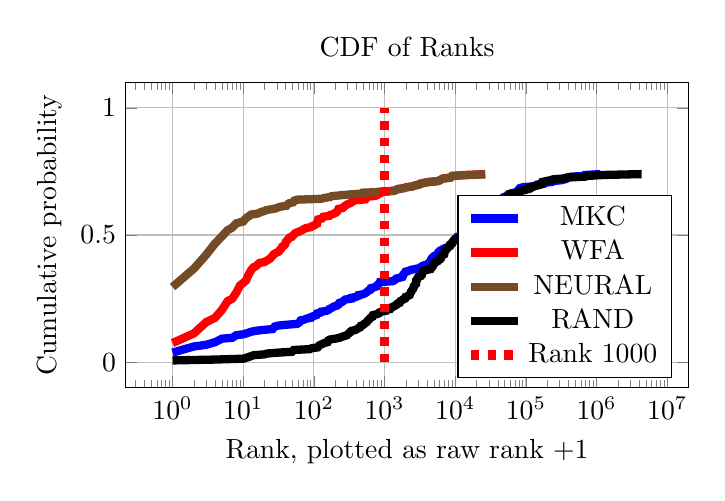
\begin{tikzpicture}
  \begin{axis}[
    width=0.72\linewidth,
  height=0.45\linewidth,
  xmode=log,
  log basis x=10,
  xlabel={Rank, plotted as raw rank $+1$},
  ylabel={Cumulative probability},
  title={CDF of Ranks},
  legend pos=south east,
  grid=major,
  ]

    \addplot+[mark=none, line width=3pt] coordinates {
      (1,0.03767123)
      (2,0.06164384)
      (3,0.06849315)
      (4,0.07876712)
      (5,0.09246575)
      (7,0.09589041)
      (8,0.10616438)
      (10,0.10958904)
      (11,0.11301370)
      (12,0.11643836)
      (13,0.11986301)
      (15,0.12328767)
      (19,0.12671233)
      (26,0.13013699)
      (28,0.14041096)
      (31,0.14383562)
      (41,0.14726027)
      (58,0.15068493)
      (63,0.15753425)
      (64,0.16095890)
      (65,0.16438356)
      (74,0.16780822)
      (78,0.17123288)
      (91,0.17465753)
      (92,0.17808219)
      (99,0.18150685)
      (108,0.18493151)
      (109,0.18835616)
      (111,0.19178082)
      (125,0.19520548)
      (127,0.19863014)
      (151,0.20205479)
      (161,0.20547945)
      (165,0.20890411)
      (184,0.21575342)
      (192,0.21917808)
      (214,0.22260274)
      (222,0.22602740)
      (223,0.22945205)
      (228,0.23287671)
      (249,0.23630137)
      (258,0.23972603)
      (278,0.24657534)
      (341,0.25000000)
      (342,0.25342466)
      (396,0.25684932)
      (424,0.26027397)
      (427,0.26369863)
      (493,0.26712329)
      (529,0.27054795)
      (553,0.27397260)
      (573,0.27739726)
      (589,0.28082192)
      (628,0.28424658)
      (636,0.28767123)
      (642,0.29109589)
      (718,0.29452055)
      (770,0.29794521)
      (778,0.30136986)
      (810,0.30479452)
      (826,0.30821918)
      (861,0.31164384)
      (867,0.31506849)
      (1304,0.31849315)
      (1376,0.32191781)
      (1414,0.32534247)
      (1463,0.32876712)
      (1640,0.33219178)
      (1799,0.33561644)
      (1819,0.33904110)
      (1821,0.34246575)
      (1854,0.34589041)
      (1903,0.34931507)
      (1970,0.35273973)
      (1992,0.35616438)
      (2207,0.35958904)
      (2357,0.36301370)
      (2686,0.36643836)
      (3097,0.36986301)
      (3321,0.37328767)
      (3361,0.37671233)
      (3531,0.38013699)
      (4054,0.38356164)
      (4206,0.38698630)
      (4223,0.39041096)
      (4373,0.39383562)
      (4455,0.39726027)
      (4517,0.40068493)
      (4631,0.40410959)
      (4632,0.40753425)
      (4731,0.41095890)
      (4958,0.41438356)
      (5057,0.41780822)
      (5533,0.42123288)
      (5647,0.42465753)
      (5679,0.42808219)
      (5740,0.43150685)
      (5906,0.43493151)
      (6086,0.43835616)
      (6469,0.44178082)
      (6721,0.44520548)
      (7140,0.44863014)
      (7920,0.45205479)
      (8276,0.45547945)
      (8554,0.45890411)
      (8698,0.46232877)
      (8782,0.46575342)
      (9046,0.46917808)
      (9159,0.47260274)
      (9473,0.47602740)
      (10005,0.47945205)
      (10083,0.48287671)
      (10176,0.48630137)
      (10544,0.48972603)
      (10711,0.49315068)
      (11811,0.49657534)
      (12062,0.50000000)
      (12283,0.50342466)
      (13236,0.50684932)
      (14344,0.51027397)
      (14414,0.51369863)
      (14510,0.51712329)
      (14995,0.52054795)
      (15071,0.52397260)
      (15356,0.52739726)
      (17180,0.53082192)
      (17231,0.53424658)
      (17387,0.53767123)
      (17695,0.54109589)
      (18522,0.54452055)
      (19287,0.54794521)
      (19919,0.55136986)
      (20273,0.55479452)
      (20463,0.55821918)
      (21741,0.56164384)
      (22392,0.56506849)
      (22579,0.56849315)
      (22665,0.57191781)
      (22728,0.57534247)
      (23154,0.57876712)
      (24775,0.58219178)
      (25574,0.58561644)
      (25588,0.58904110)
      (26959,0.59246575)
      (27020,0.59589041)
      (27120,0.59931507)
      (27470,0.60273973)
      (28124,0.60616438)
      (28535,0.60958904)
      (29384,0.61301370)
      (29770,0.61643836)
      (30782,0.61986301)
      (35286,0.62328767)
      (35362,0.62671233)
      (36281,0.63013699)
      (37928,0.63356164)
      (42111,0.63698630)
      (46758,0.64041096)
      (49229,0.64383562)
      (49744,0.64726027)
      (50222,0.65068493)
      (53522,0.65410959)
      (56356,0.65753425)
      (57107,0.66095890)
      (61827,0.66438356)
      (71578,0.66780822)
      (73835,0.67123288)
      (77346,0.67465753)
      (78487,0.67808219)
      (80081,0.68150685)
      (82264,0.68493151)
      (91862,0.68835616)
      (128602,0.69178082)
      (143381,0.69520548)
      (145199,0.69863014)
      (177352,0.70205479)
      (178434,0.70547945)
      (233866,0.70890411)
      (240246,0.71232877)
      (320307,0.71575342)
      (355812,0.71917808)
      (357216,0.72260274)
      (389140,0.72602740)
      (427904,0.72945205)
      (675222,0.73287671)
      (688859,0.73630137)
      (1125521,0.73972603)
    };
    \addlegendentry{MKC}

    \addplot+[mark=none, line width=3pt] coordinates {
      (1,0.07534247)
      (2,0.11301370)
      (3,0.15753425)
      (4,0.17465753)
      (5,0.20547945)
      (6,0.23972603)
      (7,0.25000000)
      (8,0.27397260)
      (9,0.30136986)
      (10,0.31164384)
      (11,0.32191781)
      (12,0.34589041)
      (13,0.36301370)
      (14,0.37328767)
      (15,0.37671233)
      (17,0.39041096)
      (20,0.39383562)
      (23,0.40410959)
      (24,0.40753425)
      (26,0.41780822)
      (27,0.42465753)
      (30,0.43150685)
      (32,0.43493151)
      (33,0.44178082)
      (35,0.44863014)
      (36,0.45547945)
      (38,0.45890411)
      (39,0.46232877)
      (40,0.47260274)
      (41,0.47602740)
      (42,0.47945205)
      (43,0.48287671)
      (45,0.48972603)
      (49,0.49315068)
      (50,0.49657534)
      (53,0.50342466)
      (54,0.50684932)
      (57,0.51027397)
      (62,0.51369863)
      (66,0.51712329)
      (73,0.52397260)
      (77,0.52739726)
      (90,0.53082192)
      (93,0.53424658)
      (101,0.53767123)
      (105,0.54109589)
      (111,0.54452055)
      (112,0.55136986)
      (113,0.55479452)
      (115,0.56164384)
      (130,0.56506849)
      (135,0.57191781)
      (165,0.57534247)
      (169,0.57876712)
      (185,0.58219178)
      (195,0.58561644)
      (208,0.58904110)
      (214,0.59246575)
      (216,0.59589041)
      (220,0.59931507)
      (223,0.60273973)
      (256,0.60616438)
      (264,0.60958904)
      (269,0.61301370)
      (283,0.61643836)
      (294,0.61986301)
      (333,0.62671233)
      (342,0.63013699)
      (366,0.63356164)
      (386,0.63698630)
      (537,0.64041096)
      (548,0.64383562)
      (553,0.64726027)
      (569,0.65068493)
      (737,0.65410959)
      (788,0.65753425)
      (807,0.66095890)
      (876,0.66438356)
      (902,0.66780822)
      (903,0.67123288)
      (1357,0.67465753)
      (1460,0.67808219)
      (1542,0.68150685)
      (1879,0.68493151)
      (2032,0.68835616)
      (2489,0.69178082)
      (2662,0.69520548)
      (3065,0.69863014)
      (3168,0.70205479)
      (3603,0.70547945)
      (4147,0.70890411)
      (5596,0.71232877)
      (6081,0.71575342)
      (6331,0.71917808)
      (6682,0.72260274)
      (8510,0.72602740)
      (8849,0.72945205)
      (9038,0.73287671)
      (13998,0.73630137)
      (26568,0.73972603)
    };
    \addlegendentry{WFA}

    \addplot+[mark=none, line width=3pt] coordinates {
      (1,0.29553265)
      (2,0.36769759)
      (3,0.42268041)
      (4,0.46735395)
      (5,0.49484536)
      (6,0.51890034)
      (7,0.52920962)
      (8,0.54639175)
      (10,0.55326460)
      (11,0.56701031)
      (12,0.57388316)
      (13,0.58075601)
      (16,0.58419244)
      (18,0.59106529)
      (20,0.59450172)
      (21,0.59793814)
      (25,0.60137457)
      (29,0.60481100)
      (31,0.60824742)
      (34,0.61168385)
      (41,0.61512027)
      (43,0.62199313)
      (45,0.62542955)
      (51,0.62886598)
      (52,0.63230241)
      (53,0.63573883)
      (58,0.63917526)
      (128,0.64261168)
      (141,0.64604811)
      (170,0.64948454)
      (178,0.65292096)
      (322,0.65979381)
      (482,0.66323024)
      (491,0.66666667)
      (988,0.67010309)
      (1357,0.67353952)
      (1460,0.67697595)
      (1542,0.68041237)
      (1879,0.68384880)
      (2032,0.68728522)
      (2489,0.69072165)
      (2662,0.69415808)
      (3065,0.69759450)
      (3168,0.70103093)
      (3603,0.70446735)
      (4147,0.70790378)
      (5596,0.71134021)
      (6081,0.71477663)
      (6331,0.71821306)
      (6682,0.72164948)
      (8510,0.72508591)
      (8849,0.72852234)
      (9038,0.73195876)
      (13998,0.73539519)
      (26568,0.73883162)
    };
    \addlegendentry{NEURAL}

    \addplot+[mark=none, line width=3pt] coordinates {
      (1,0.00684932)
      (4,0.01027397)
      (10,0.01369863)
      (12,0.02054795)
      (14,0.02739726)
      (20,0.03082192)
      (22,0.03424658)
      (32,0.03767123)
      (49,0.04109589)
      (52,0.04794521)
      (88,0.05136986)
      (93,0.05479452)
      (113,0.05821918)
      (115,0.06164384)
      (118,0.06506849)
      (123,0.06849315)
      (133,0.07191781)
      (141,0.07534247)
      (156,0.07876712)
      (158,0.08219178)
      (160,0.08561644)
      (168,0.08904110)
      (201,0.09246575)
      (231,0.09589041)
      (246,0.09931507)
      (270,0.10273973)
      (294,0.10616438)
      (301,0.10958904)
      (313,0.11301370)
      (325,0.11643836)
      (328,0.11986301)
      (340,0.12328767)
      (388,0.12671233)
      (408,0.13013699)
      (424,0.13356164)
      (454,0.13698630)
      (466,0.14041096)
      (468,0.14383562)
      (503,0.14726027)
      (515,0.15068493)
      (536,0.15410959)
      (561,0.15753425)
      (572,0.16095890)
      (582,0.16438356)
      (605,0.16780822)
      (614,0.17123288)
      (635,0.17465753)
      (670,0.17808219)
      (674,0.18150685)
      (684,0.18493151)
      (768,0.18835616)
      (829,0.19178082)
      (842,0.19520548)
      (897,0.19863014)
      (1034,0.20205479)
      (1040,0.20547945)
      (1206,0.20890411)
      (1239,0.21232877)
      (1256,0.21575342)
      (1341,0.21917808)
      (1422,0.22260274)
      (1484,0.22602740)
      (1508,0.22945205)
      (1622,0.23287671)
      (1626,0.23630137)
      (1664,0.23972603)
      (1765,0.24315068)
      (1813,0.24657534)
      (1954,0.25000000)
      (1977,0.25342466)
      (1991,0.25684932)
      (2136,0.26027397)
      (2265,0.26369863)
      (2279,0.26712329)
      (2317,0.27054795)
      (2356,0.27397260)
      (2365,0.27739726)
      (2431,0.28082192)
      (2460,0.28424658)
      (2525,0.28767123)
      (2563,0.29109589)
      (2572,0.29452055)
      (2584,0.29794521)
      (2667,0.30136986)
      (2695,0.30479452)
      (2791,0.30821918)
      (2804,0.31506849)
      (2808,0.32191781)
      (2896,0.32534247)
      (2914,0.32876712)
      (2936,0.33219178)
      (2993,0.33561644)
      (3283,0.33904110)
      (3359,0.34246575)
      (3370,0.34589041)
      (3421,0.34931507)
      (3443,0.35273973)
      (3495,0.35616438)
      (3549,0.35958904)
      (3997,0.36301370)
      (4501,0.36643836)
      (4557,0.36986301)
      (4672,0.37328767)
      (4809,0.37671233)
      (4858,0.38013699)
      (4891,0.38356164)
      (4955,0.38698630)
      (5183,0.39041096)
      (5241,0.39383562)
      (5637,0.39726027)
      (5695,0.40068493)
      (6095,0.40410959)
      (6263,0.40753425)
      (6340,0.41095890)
      (6374,0.41438356)
      (6444,0.41780822)
      (6510,0.42123288)
      (6996,0.42465753)
      (7037,0.42808219)
      (7085,0.43150685)
      (7128,0.43493151)
      (7130,0.43835616)
      (7451,0.44178082)
      (7615,0.44520548)
      (7770,0.44863014)
      (7902,0.45205479)
      (8311,0.45547945)
      (8336,0.45890411)
      (8430,0.46232877)
      (8952,0.46575342)
      (9112,0.46917808)
      (9194,0.47260274)
      (9355,0.47602740)
      (9494,0.47945205)
      (9783,0.48287671)
      (10378,0.48630137)
      (11892,0.48972603)
      (12230,0.49315068)
      (12554,0.49657534)
      (12589,0.50000000)
      (12888,0.50342466)
      (13024,0.50684932)
      (13071,0.51027397)
      (13178,0.51369863)
      (13512,0.51712329)
      (14208,0.52054795)
      (14647,0.52397260)
      (14663,0.52739726)
      (15332,0.53082192)
      (15908,0.53424658)
      (16720,0.53767123)
      (17154,0.54109589)
      (18163,0.54452055)
      (20212,0.54794521)
      (20425,0.55136986)
      (20927,0.55479452)
      (21469,0.55821918)
      (22636,0.56164384)
      (25070,0.56506849)
      (25260,0.56849315)
      (25748,0.57191781)
      (25901,0.57534247)
      (26604,0.57876712)
      (27276,0.58219178)
      (27599,0.58561644)
      (27818,0.58904110)
      (28649,0.59246575)
      (29192,0.59589041)
      (29816,0.59931507)
      (31144,0.60273973)
      (31798,0.60616438)
      (33290,0.60958904)
      (35029,0.61301370)
      (35278,0.61643836)
      (37482,0.61986301)
      (37967,0.62328767)
      (38156,0.62671233)
      (39213,0.63013699)
      (39886,0.63356164)
      (40022,0.63698630)
      (44812,0.64041096)
      (45399,0.64383562)
      (48179,0.64726027)
      (55360,0.65068493)
      (56741,0.65410959)
      (58495,0.65753425)
      (59275,0.66095890)
      (70270,0.66438356)
      (79371,0.66780822)
      (83862,0.67123288)
      (84156,0.67465753)
      (100049,0.67808219)
      (110475,0.68150685)
      (110884,0.68493151)
      (124036,0.68835616)
      (127452,0.69178082)
      (146822,0.69520548)
      (162444,0.69863014)
      (162561,0.70205479)
      (171230,0.70547945)
      (171816,0.70890411)
      (194431,0.71232877)
      (222344,0.71575342)
      (243777,0.71917808)
      (344517,0.72260274)
      (377343,0.72602740)
      (676363,0.72945205)
      (781342,0.73287671)
      (1250401,0.73630137)
      (4338854,0.73972603)
    };
    \addlegendentry{RAND}

    \addplot+[red, dashed, line width=3.4pt, mark=none] coordinates {
      (1000,0)
      (1000,1)
    };
    \addlegendentry{Rank 1000}

  \end{axis}
\end{tikzpicture}}

% =========================================================
    \mysection{Takeaways \& Next Steps}

    \null\hspace*{2.8cm}\begin{minipage}[c]{0.86\columnwidth}
        \renewcommand\labelitemi{$\vcenter{\hbox{\small\bullet}}$}
        \begin{itemize}[labelsep=0.8cm]
          \item A fixed-parameter $\langle k, |\mathbb{T}|\rangle$ tractable embedding from a syntax-directed type system to a CFG with soundness and completeness guarantees.
          \item Intersection with an acyclic FSA yields a star-free regular expression.
          \item Brzozowski derivatives enable incremental autoregressive decoding.
          \item Future work: lazy CNF materialization, quotienting (e.g., $\alpha$-equivalence), richer type theories (subtyping, polymorphism, substructural constraints).
        \end{itemize}
    \end{minipage}

  \end{multicols}

  \bottombox{
    \phantom{
    \begin{minipage}[c][0.1\paperheight][c]{0.1\textwidth}
      \qrcode[height=2.6in]{https://tidyparse.github.io/}
    \end{minipage}
    \begin{minipage}[c][0.1\paperheight][c]{0.1\textwidth}
      
\includegraphics[height=2.6in]{../figures/tidyparse_logo.png}
    \end{minipage}
    \hspace{-4cm}
    \begin{minipage}[c][0.1\paperheight][c]{0.1\textwidth}
      
\includegraphics[height=3in]{../figures/mcgill.png}
    \end{minipage}
    \hspace{2cm}
    \begin{minipage}[c][0.1\paperheight][c]{0.1\textwidth}
      
\includegraphics[height=3.2in]{../figures/mila.png}
    \end{minipage}}
  }
\end{poster}
\end{document}